\chapter{Implementação}

Após a apresentação da metodologia, este capítulo tem por objetivo demonstrar a aplicação desta abordagem em diferentes exemplos. Para esta demonstração foram escolhidos cenários apresentados em trabalhos que SMA foram modelados de acordo com a organização $\mathcal{M}$oise$^{+}$. A escolha destes cenários se baseou na relevância dos autores, apresentarem a documentação das especificações necessárias para o desenvolvimento da metodologia e nível de complexidade.

\section{Writing paper}

\subsection{Descrição do cenário}

Este primeiro exemplo foi apresentado no trabalho \cite{kitio2008organisational} e estendido em \cite{hubner2011normative}, e representa um grupo de agentes com objetivo de escrever um artigo. A especificação estrutural desta organização descreve que ela é composta por apenas um grupo \textit{wpgroup} e este grupo possui dois papéis \textit{escritor} e \textit{editor} e ambos são sub-papéis de \textit{autor} Figura \ref{fig:writing-paper-estrutural}.
    
\begin{figure}[ht]
\centering
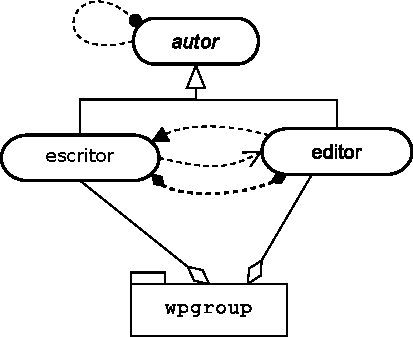
\includegraphics[scale=0.7]{imagens/5-writing-paper-estrutural.pdf}
\caption{Especificação estrutural \textit{Writing paper}. \cite{hubner2011normative}}
\label{fig:writing-paper-estrutural}
\end{figure}
    
Para coordenar este grupo de agentes a atingir sua meta, um esquema funcional é definido Figura \ref{fig:writing-paper-funcional}. Neste esquema primeiro um agente que assume a missão \textit{mMan} deve escrever uma versão de rascunho do artigo (\textit{fdv}), contendo como sub-metas escrever um título (\textit{wtitle}), um resumo (\textit{wabs}) e o título das seções (\textit{wsectitle}) sendo necessário atingir os objetivos nesta sequência. A segunda ramificação denominada \textit{sv}, versão de submissão é composta pelas metas \textit{wsec} escrever seção, e a finalização do artigo composta por duas metas em paralelo, escrever a conclusão \textit{wcon} e escrever as referências \textit{wref}.
    
\begin{figure}[ht]
\centering
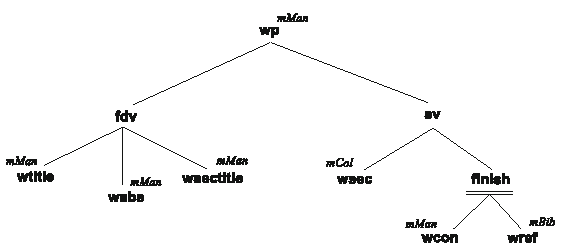
\includegraphics[scale=1.3]{imagens/5-writing-paper-funcional.pdf}
\caption{Especificação funcional \textit{Writing paper}. \cite{hubner2011normative}}
\label{fig:writing-paper-funcional}
\end{figure}

A Tabela \ref{tab:writing-paper-deontica} representa a especificação deôntica que define as permissões e obrigações dos papéis que assumem as missões. Estas missões são definidos por \textit{mMan} gerenciamento geral do projeto, composta por quatro metas, \textit{mCol} colaboração na escrita do conteúdo  e a missão \textit{mBib} em que o agente que assumir deverá reunir e escrever as referências do artigo.

\begin{table}[ht]
\centering
\caption{Especificação deôntica \textit{Writing paper}. \cite{hubner2011normative}}
\label{tab:writing-paper-deontica}
\begin{tabular}{@{}lll@{}}
\toprule
papel       & relação deôntica  & missão                        \\ \midrule
editor      & permissão         & \textit{mMan}                          \\
escritor    & obrigação         & \textit{mCol}                          \\
escritor    & obrigação         & \textit{mBib}                          \\
\bottomrule
\end{tabular}
\end{table}

\subsection{Implementação}

Seguindo a etapas da metodologia definimos a ordem de execução das metas.
    
    
\section{\textit{Multi-Agent Programming Contest- Agents on Mars}}

\subsection{Descrição do cenário}

Este cenário faz parte da \textit{Multi-Agent Programming Contest} \footnote[1]{https://multiagentcontest.org/}, um evento anual que tem o objetivo de estimular a pesquisa na área de desenvolvimento e programação de SMA. Através da competição é possível avaliar e comparar diferentes aspectos dos sistemas desenvolvidos, identificando problemas, coletando \textit{benchmarks} e reunindo casos de teste que podem servir como referência para testar linguagens de programação multiagente, plataformas e ferramentas \cite{koster2012multi, ahlbrecht2013multi}.

Neste ano o cenário da competição é Marte, onde os competidores deverão desenvolver agentes inteligentes autônomos para localizar poços de água, ocupar
as melhores zonas de Marte e sabotar seus rivais para conseguir seu objetivo ou para defender si mesmos. Neste contexto foi utilizado a solução da equipe SMADAS-UFSC que venceu a competição no ano de 2013 e desenvolveu a solução utilizando Jason, Cartago e $\mathcal{M}$oise$^{+}$ \cite{zatelli2013smadas, ahlbrecht2013multi}.

\begin{figure}[ht]
  \centering
  \subfigure[]{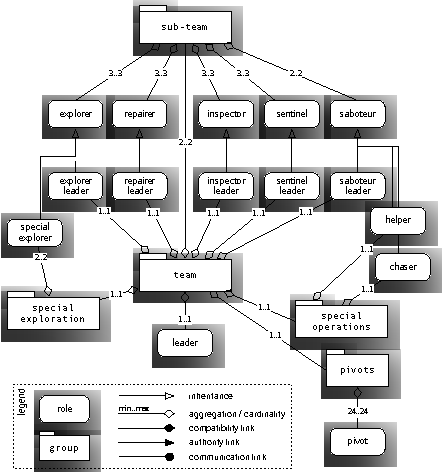
\includegraphics[width=0.45\textwidth]{imagens/marte-estrutural.pdf}\label{fig:marte-estrutural}}
  \subfigure[]{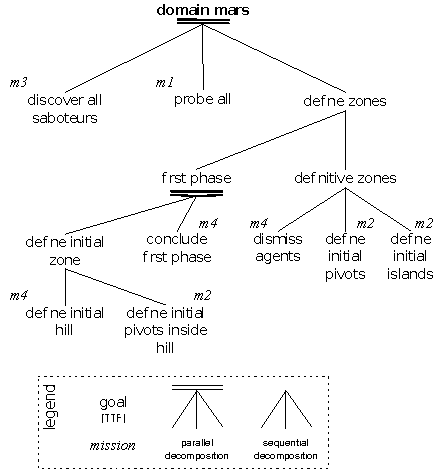
\includegraphics[width=0.45\textwidth]{imagens/marte-funcional.pdf}\label{fig:marte-funcional}}
  \caption{Agentes em Marte}
  \label{fig:marte}
\end{figure}


\begin{table}[ht]
\centering
\caption{Especificação deôntica \textit{Agentes em Marte}. \cite{zatelli2013smadas}}
\label{tab:marte-deontica}
\begin{tabular}{@{}llll@{}}
\toprule
norma   & papel         & relação deôntica  & missão                    \\ \midrule
n1      & explorer          & obrigação         & \textit{m1}               \\
n2      & sentinelLeader    & obrigação         & \textit{m2}               \\
n3      & inspector         & obrigação         & \textit{m3}               \\
n4      & explorerLeader    & obrigação         & \textit{m4}               \\
\bottomrule
\end{tabular}
\end{table}
  
\subsection{Implementação}